\section{Exploring Covariance Functions}
The behaviour of the covariance function and its resulting covariance matrix is crucial to understanding the behaviour of the Gaussian process - the covariance matrix appears in every term of the predictive distribution and the marginal likelihood. In particular, the choice of covariance function affects the smoothness of the overall GP. This section describes the mechanisms that the covariance function has at its disposal to vary smoothness, namely its degree of differentiability and the choice of length scale. We investigate in detail the stationary family of covariance functions, discuss why they are the most widely used, and develop a new tool to analyse them. Finally, we introduce the most widespread stationary covariance functions, their properties, and the types of data they are best suited for.

% We have seen that a covariance function is the crucial ingredient in a Gaussian process predictor, as it encodes our assumptions about the function which we wish to learn. From a slightly different viewpoint it is clear that in supervised learning the notion of similarity between data points is crucial; it is a basic similarity assumption that points with inputs x which are close are likely to have similar target values y, and thus training points that are near to a test point should be informative about the prediction at that point. Under the Gaussian process view it is the covariance function that defines nearness or similarity.

% An arbitrary function of input pairs x and x′ will not, in general, be a valid valid covariance functionscovariance function.1 The purpose of this chapter is to give examples of some commonly-used covariance functions and to examine their properties. Section 4.1 defines a number of basic terms relating to covariance functions. Section 4.2 gives examples of stationary, dot-product, and other non-stationary covariance functions, and also gives some ways to make new ones from old. Section 4.3 introduces the important topic of eigenfunction analysis of covariance functions, and states Mercer’s theorem which allows us to express the covariance function (under certain conditions) in terms of its eigenfunctions and eigenvalues. 

\subsection{Characteristics of covariance functions \cite{gp-ml}}

\subsubsection{Covariance matrices}
The inner product representations of the covariance for our Bayesian model in function-space \ref{eq:gp_bayesian}, weight-space \ref{eq:alt_predictive_gaussian_phi}, and covariance matrices in general can be represented as a Gram matrices. Given a vector of input points ${X_i | i = 1, ..., n}$ and a covariance function $k$, a Gram matrix $K$ is the $n \times n$ matrix whose $(i,j)$-th entry is $k(x_i, x_j)$. This requires any proposed covariance matrix to exhibit the properties of a Gram matrix, namely symmetry and positive semidefiniteness:

\begin{equation*}
    \begin{aligned}
        K_{ij} = K_{ji} \\
        X^T K X \geq 0
    \end{aligned}
\end{equation*}

Symmetry is inherent from the inner product property since inner products are symmetric, i.e. $X_i^T X_j = X_j^T X_i$, and imposes $cov(X_i, X_j) = cov(X_j, X_i)$. $K$ satisfies positive semidefiniteness if, for any vector $V$ of inputs, $V^T K V \geq 0$ since:
\begin{equation*}
    V^T K V = (K V)^T (K V) = ||K V||^2 \geq 0
\end{equation*}
This means that the covariance matrix must not produce negative variances for any linear combination of inputs.


\subsubsection{Eigenvalue and eigenfunctions of covariance matrices}

\paragraph{Integral operators}
If we wanted to multiply a vector $\Phi$ by a matrix $K(X,X')$, we would use the following matrix-vector multiplication to produce a discrete vector $[K \phi]$:
\begin{equation*}
    [K \phi]_i = \sum_{j=1}^{n} K_{ij} \Phi_j
\end{equation*}
If we wanted to multiply a function $\phi(x)$ by our matrix $K(X,X')$, we could use an "integral operator" $K$ to produce a new contnuous function $[K\phi](x')$:
\begin{equation*}
    [K\phi](x') = \int K(x, x') \phi(x) dx
\end{equation*}
This specific usage of $K(X,X')$ is where covariance matrices are known as kernels, but the terms "kernel" and "covariance matrix" are used interchangably outside of this context. For example, using the linear kernel $K(x, x') = x \cdot x'$, a function $\phi(x) = x^2$, and the limits of our domain $a = 0$ and $b = 1$:
\begin{equation*}
    [K\phi](x') = \int x \cdot x' x^2 dx = x' \int_0^1 x^3 dx = x' [ \frac{x^4}{4} ]_0^1 = x' \cdot \frac{1}{4}
\end{equation*}
$[K\phi](x')$ becomes $x'$ scaled by the RHS integral - the first term depends on our choice of kernel, and the size of the scale depends on $\phi(x)$ and $a, b$.

We can refer to some vector $\Phi$ as the eigenvector and $\lambda$ as the eigenvalue of $K$ if it obeys this equation:
\begin{equation*}
    [K \Phi] = \lambda \Phi
\end{equation*}
Since our integral operator $K$ is like an infinite-dimensional matrix whose entries are $k(x, x')$, we can refer to a function $\phi(x)$ as the eigenfunction and $\lambda$ as the eigenvalue of our integral operator $K$ if:
\begin{equation*}
    \int K(x, x') \phi(x) d\mu(x) = \lambda \phi(x')
\end{equation*}
where $\mu$ is some measure over the domain of $x$ upon which the integration will occur thus defining the limits of integration $a, b$. 

\paragraph{Mercer's theorem}
If our kernel satisfies the conditions of a Gram matrix (i.e. symmetry and positive semidefiniteness) and our measure $\mu$ is any compact subset $C \subset \mathbb{R}^n$ (e.g. the probability space $[0,1]$), then it conforms to Mercer's theorem. Mercer's theorem states that these eigenvalues $[\lambda_i]_{i=1}^\infty$ are non-negative and decay to zero, and our kernel itself can be decomposed into a sum of eigenfunctions $\phi_i$ and eigenvalues $\lambda_i$:
\begin{equation} \label{eq:gp_mercer}
    K(X, X') = \sum_{i=1}^{\infty} \lambda_i \phi_i(X) \phi_i(X')
\end{equation}
A kernel with infinite rank, or a covariance function that has infinite basis functions (e.g. SE), is called a nondegenerate kernel, else it is degenerate. For example, our $N$-dimensional linear kernel $K(X, X') = X \cdot X'$ results in a degenerate kernel with at most $N$ non-zero eigenvalues.


\subsubsection{Varying the length scale}
Our covariance functions has some hyperparameters, e.g. the full form of SE in one dimension contains some free parameters $\sigma^2_f$, $\sigma^2_n$, and $l$:
\begin{equation*}
    k_y(x,x') = \sigma^2_f \exp\left(-\frac{1}{2}\frac{|x - x'|^2}{l^2}\right) + \sigma^2_n\delta_{x,x'}
\end{equation*}
Note that our covariance function is for $k_y$ as it is for the noisy targets $y$, not the function $f$. $\sigma^2_f$ is the signal variance, which controls the overall scale of the function. $\sigma^2_n$ is the noise variance, which controls the amount of noise in the observations. $\delta_{X,X'}$ is the Kronecker delta which represents our independence of noise assumption.

$l$ is a "length scale" hyperparameter that controls how sensitive our functions are - if we specify a lower $l$, we can "artificially" get a high $k(X,X')$. One way to determine $l$ is by the expected number of "upcrossings" that our kernel is expected to make for a given level $u$. A function performs an upcrossing for $u$ when $u = f(x)$ and $dy/dx > 0$. For example, with $u = 2$ and $y = x^2$, there exists one upcrossing at $(2, \sqrt{2})$ where $dy/dx = 4$, and a downcrossing at $(2, -\sqrt{2})$ where $dy/dx = -4$. For our zero-mean Gaussian processes, the expected number of upcrossings of our (stationary) kernel for a level $ 0 < u < 1$ is:
\begin{equation*}
    \mathbb{E}[N_u] = \frac{1}{2\pi} \sqrt{\frac{-k''(0)}{k(0)}} \exp \left(-\frac{u^2}{2k(0)}\right)
\end{equation*}
We can empirically count the number of upcrossings between 0 and 1 $\hat{N}_u$ and set this equal to the expected number of upcrossings to get a value for $l$:
\begin{equation} \label{eq:general_l}
    \frac{1}{2\pi} \sqrt{\frac{-k''(0)}{k(0)}} \exp \left(-\frac{u^2}{2k(0)}\right) = \hat{N}_u
\end{equation}

A large amount of upcrossings implies our data-generating function wiggles rapidly, so our $l$ becomes smaller to produce a covariance function that in turn produces more flexible functions.

\subsubsection{Mean square continuity and differentiability}
To understand how smooth the functions drawn from a Gaussian process are, we need to understand how differentiable and continuous they are. A more differentiable function implies that the function contains higher order polynomials which makes it smoother, and a continuous function avoids any reductions in smoothness produced by discontinuities.

Because the functions drawn from the Gaussian distribution are random functions between datapoints, there are infinitely many possible functions and determining if they are all continuous or differentiable is impossible. TODO 

% We are l Instead, we can examine if the covariance function responsible for producing these functions is differentiable and continuous.

% The quadratic term in our limit means our mean squared errors will also vary continuously, so we avoid wild "swings" in uncertainty when moving away from training data points in the input space. More importantly, it allows the error term to be expanded directly into kernel terms: 

\paragraph{Continuity}
Let $x$ be an infinite-length vector of inputs $x_1, x_2, ...$ whose values linearly approach some stable fixed point $x_*$ as the sequence progresses. Formally:
\begin{equation*}
    \lim_{k \to \infty} |x_k - x_*| = 0
\end{equation*}

A regular function $f$ is continuous at $x_*$ if three conditions are met. $x_*$ must exist in the domain of $f$, e.g. $f(X) = 1/x$ is not continuous at $f(0)$ because $0$ is not in the domain of $f$. There must be a single limit the function approaches.
\begin{equation*}
    f(X) = \begin{cases}
        0 & \text{if } X < 0 \\
        1 & \text{if } X > 0 \\
        2 & \text{if } X = 0
    \end{cases}
\end{equation*}
In this example, at $f(0)$ $x$ is not continuous at $x = 0$ since $f$ approaches both $0$ and $1$. This single limit needs to be the same as the function evaluation at the limit. If we removed the $0 \text{ if } X < 0$ case to produce a single limit, it would still not be continuous at $x = 0$ since the limit would be $1$ but $f(0) = 2$. Formally summarising these three ideas:
\begin{equation*}
    \lim_{x \to x_*} |f(x) - f(x_*)| = 0
\end{equation*}

A Gaussian process $f$ is MS continuous at $x_*$ if the expected function evaluations $E[f(x)]$ quadratically approach $f(x_*)$ as $x \to x_*$. Formally:
\begin{equation*}
    \lim_{x \to x_*} \mathbb{E}[(f(x) - f(x_*))^2] = 0
\end{equation*}

Thanks to the quadratic term, we can expand our error term directly into kernel terms. The covariance function $k$ is defined as the expected value of the product of two function evaluations:
\begin{equation*}
    \begin{aligned}
        \mathbb{E}[(f(x) - f(x_*))^2] = \mathbb{E}[f(x)^2] + \mathbb{E}[f(x_*)^2] - 2\mathbb{E}[f(x)f(x_*)] \\
        = k(x, x) + k(x_*, x_*) - 2k(x, x_*)
    \end{aligned}
\end{equation*}
Using this expansion in our definition of MS continuity: 
\begin{equation} \label{eq:ms_continuity}
    \lim_{x \to x_*} | k(x, x) - 2k(x, x_*) + k(x_*, x_*) | = 0
\end{equation}
Because $x_*$ is given, $k(x_*, x_*)$ is a constant. This limit requires that both $k(x, x)$ and $k(x, x_*) \to k(x_*, x_*)$ as $x \to x_*$, which is the very definition of continuity of $k$ at $x_*$ - they guarantee that $x_*$ is in the domain of $k$, that it has a single limit, and this limit of $k(x, x_*)$ is $k(x_*, x_*)$ as $x \to x_*$. Therefore, a Gaussian process is MS continuous at $x_*$ if and only if the covariance function $k$ is continuous at $x_*$.  

\paragraph{Differentiability}
$f$ is MS differentiable at $x_*$ in the $i$th direction of our input vector $X$ if:
\begin{equation*}
    \lim_{h \to 0} \mathbb{E} \left[| \frac{(f(x_* + h e_i) - f(x_*))}{h} - \frac{\partial f}{\partial x_{*i}}(x_*) |\right]^2 = 0
\end{equation*}
$e_i = (0_0, ..., 0_{i-1}, 1_i, 0_{i+1}, ..., 0_n)$ is a unit vector that constrains the change in $x$ to only the $i$th dimension. We assume $m(x_*) = 0$ for simplicity, but a non-zero mean does not change the structure of this proof and leads to the same result.

Expanding and creating simplifying $A$ and $B$ terms to represent the limit and the proposed derivative respectively:
\begin{equation*}
    \begin{aligned}
        \lim_{h \to 0} \mathbb{E} \left[(A_h - B)^2\right] = \mathbb{E}[A_h^2] + \mathbb{E}[B^2] - 2\mathbb{E}[A_h B] = 0 \\
        A_h = \frac{f(x_* + h e_i) - f(x_*)}{h} \\
        B = \frac{\partial f}{\partial x_{*i}}(x_*)
    \end{aligned}
\end{equation*}
Similar to MS continuity, we expand $A_h^2$ into kernel terms:
\begin{equation} \label{eq:msd_a}
    \mathbb{E}[A_h^2] = \frac{1}{h^2} \left( k(x_* + h e_i, x_* + h e_i) + k(x_*, x_*) - 2k(x_* + h e_i, x_*) \right)
\end{equation}
$k(x_*,x_*)$ is a constant, but the other terms vary with $h$. We can use a second-order Taylor series to approximate these terms if $k$ is twice continuously differentiable at $x_*$. Starting with the univariate $k(x_* + h e_i, x_*)$:
\begin{equation*}
    \begin{aligned}
        k(x_* + h e_i, x_*) = \\
        k(x_*, x_*) \\
        + h [\partial_{u_i}k](x_*, x_*) \\
        + \frac{h^2}{2} [\partial_{u_i u_i}^2k] (x_*, x_*) \\
        + O(h^3)
    \end{aligned}
\end{equation*}
$u_i$ and $v_i$ denote the first $x_* + h e_i$ and second $x_*$ arguments respectively in the $i$th direction. TODO explain $O$ and why it's in terms of $h^3$
Then, the multivariate $k(x_* + h e_i, x_* + h e_i)$:
\begin{equation*}
    \begin{aligned}
        k(x_* + h e_i, x_* + h e_i) = \\
        k(x_*, x_*) \\
        + h [\partial_{u_i}k + \partial_{v_i}k](x_*, x_*) \\
        + \frac{h^2}{2} [\partial_{u_i u_i}^2 k + \partial_{u_i v_i}^2 k + \partial_{v_i v_i}^2 k](x_*, x_*) \\
        + O(h^3) 
    \end{aligned}
\end{equation*}
Substituting these approximations into \ref{eq:msd_a}:
\begin{equation*}
    \begin{aligned}
        \mathbb{E}[A^2_h] = \frac{1}{h^2} \\
        k(x_*, x_*) + k(x_*, x_*) - 2k(x_*, x_*) \\
        + h [\partial_{u_i}k + \partial_{v_i}k](x_*, x_*) - 2h[\partial_{u_i}k](x_*, x_*) \\
        + \frac{h^2}{2} [\partial_{u_i u_i}^2 k + \partial_{u_i v_i}^2 k + \partial_{v_i v_i}^2 k](x_*, x_*) - 2\frac{h^2}{2} [\partial_{u_i u_i}^2k](x_*, x_*) \\
        + O(h^3)
    \end{aligned}
\end{equation*}
The constant $k(x_*, x_*)$ terms cancel and the $O(h^3)$ remainders combine but remain the same order. 

We can combine the linear partial derivatives to form a single function $[\partial_{u_i}k + \partial_{v_i}k - 2\partial_{v_i}k]$. Thanks to the symmetry of the covariance matrix inherited from the Gram matrix, $k(u,v) = k(v,u)$ and $\partial_{u_i}k = \partial_{v_i}k$ and substituting in either into our linear term cancels it completely. 

Similarly, we can combine the quadratic derivatives:
\begin{equation*}
    E[A^2] = \frac{1}{h^2} \frac{h^2}{2}[\partial_{u_i u_i}^2 k + \partial_{u_i u_i}^2 k + \partial_{v_i v_i}^2k](x_*,x_*) - h^2[\partial_{u_i v_i}^2 k](x_*, x_*)
\end{equation*}
Cancelling $\frac{1}{h^2}$ and $\frac{h^2}{2}$ and simplifying:
\begin{equation*}
    \begin{aligned}
    = [\partial_{u_i v_i}^2 k + \partial_{u_i u_i}^2 k + \partial_{v_i v_i}^2k - \partial_{u_i v_i}^2 k](x_*, x_*) \\
    = [\partial_{u_i u_i}^2 k + \partial_{u_i v_i}k - \partial_{v_i v_i}^2 k](x_*, x_*)
    \end{aligned}
\end{equation*}
Similarly to the linear terms, using the symmetry of $k$ to cancel $\partial_{u_i u_i}^2$ and $\partial_{v_i v_i}^2$ yields the final expression for $\mathbb{E}[A_h^2$:
\begin{equation} \label{eq:msd_a_final}
    \mathbb{E}[A_h^2] = \partial_{u_i v_i}^2 k(x_*,x_*) + O(h^3) 
\end{equation}

Because $B$ is Gaussian, its square is simply its variance:
\begin{equation*}
    \begin{aligned}
        \mathbb{E}[B^2] = \text{Var}\left(\frac{\partial f}{\partial x_{*i}}(x_*)\right) \\
        = \text{Cov} \left(\frac{\partial f}{\partial x_{*i}}(x_*), \frac{\partial f}{\partial x_{*i}}(x_*) \right) \\
    \end{aligned}
\end{equation*}
We can substitute our regular limit definition of differentiability outside of MS space, with different small increments $h$ and $h'$:
\begin{equation*}
    = \text{Cov} \left(\frac{f(x_* + h e_i) - f(x_*)}{h}, \frac{f(x_* + h' e_i) - f(x_*)}{h'} \right)
\end{equation*}
The $h$ and $h'$ denominators merely scale the covariance, so we can take them out of the covariance expression:
\begin{equation*}
    = \frac{1}{hh'} \text{Cov} \left(f(x_* + h e_i) - f(x_*), f(x_* + h' e_i) - f(x_*) \right)
\end{equation*}
Using additivity TODO explain:
\begin{equation*}
    \mathbb{E}[B^2] = \frac{1}{hh'} \left( k(x_* + h e_i, x_* + h' e_i) - k(x_*, x_* + h' e_i) - k(x_* + h e_i, x_*) + k(x_*, x_*) \right)
\end{equation*}
We already have $k(x_* + h e_i, x_*)$ from \ref{eq:uni_taylor_a} directly, and $k(x_*, x_* + h e_i)$ by symmetry and substituting $h'$ for $h$. Our multivariate Taylor series $k(x_* + h e_i, x_* + h' e_i)$ looks similar to \ref{eq:multi_taylor_a}:
\begin{equation*}
    \begin{aligned}
        k(x_* + h e_i, x_* + h' e_i) = \\
        k(x_*, x_*) \\
        + h [\delta_{u_i}k](x_*, x_*) 
        + h' [\delta_{v_i}k](x_*, x_*) \\
        + \frac{h^2}{2} [partial_{u_i u_i}^2k](x_*, x_*) \\
        + hh' [\partial_{u_i v_i}^2k](x_*, x_*) \\
        + \frac{h'^2}{2} [\partial_{v_i v_i}^2k](x_*, x_*) \\
        + O(||(h,h')||^3)
    \end{aligned}
\end{equation*}

Substituting these results into $\mathbb{E}[B^2]$:
\begin{equation*}
    \begin{aligned}
        \mathbb{E}[B^2] = \frac{1}{hh'} \\
        k(x_*,x_*) \\
        + k(x_*,x_*) + k(x_*,x_*) - k(x_*,x_*) \\
        + h [\delta_{u_i}k](x_*, x_*) - h [\delta_{u_i}k](x_*, x_*) \\
        + h' [\delta_{v_i}k](x_*, x_*) - h' [\delta_{v_i}k](x_*, x_*) \\
        + \frac{h^2}{2} [\partial_{u_i u_i}^2k](x_*, x_*) -  \frac{h^2}{2} [\partial_{u_i u_i}^2k](x_*, x_*) \\
        + hh' [\partial_{u_i v_i}^2k](x_*, x_*) \\
        + \frac{h'^2}{2} [\partial_{v_i v_i}^2k](x_*, x_*) - \frac{h'^2}{2} [\partial_{v_i v_i}^2k](x_*, x_*) \\
        + O(h^3) + O(h'^3) + O(||(h,h')||^3) \\
    \end{aligned}
\end{equation*}
All constant, linear $h$ and $h'$, and $h^2$ and $h'^2$ terms cancel, leaving the mixed term and the remainders. $\frac{1}{hh'}$ cancel and the remainders can be combined since TODO:
\begin{equation} \label{eq:msd_b_final}
    \mathbb{E}[B^2] = \partial_{u_i v_i}^2 k(x_*, x_*) + O(h^2)
\end{equation}

For $\mathbb{E}[A_h B]$, assuming zero-mean:
\begin{equation*}
    \mathbb{E}[A_h B] = \text{Cov} \left( \frac{f(x_* + h e_i) - f(x_*)}{h}, \frac{\partial f}{\partial x_{*i}}(x_*) \right)
\end{equation*}
Similarly to $B$, we can remove the scaling factor $\frac{1}{h}$:
\begin{equation*}
    = \frac{1}{h} \text{Cov} \left( f(x_* + h e_i) - f(x_*), \frac{\partial f}{\partial x_{*i}}(x_*) \right)
\end{equation*}
By linearity of covariance TODO elabourate:
\begin{equation*}
    = \frac{1}{h} \left[ \text{Cov} (f(x_* + h e_i), \frac{\partial f}{\partial x_{*i}}(x_*) ) - \text{Cov} (f(x_*), \frac{\partial f}{\partial x_{*i}}(x_*)) \right]
\end{equation*}

A fundamental identities for Gaussian fields TODO elabourate is:
\begin{equation*}
    \begin{aligned}
        \text{Cov}(f(u), \delta_{u_i} f(v)) = \delta_{u_i} k(u, v) \\
    \end{aligned}
\end{equation*}
Applying it to both terms:
\begin{equation*}
    \begin{aligned}
        \text{Cov}(f(x_* + h e_i), \frac{\partial f}{\partial x_{*i}}(x_*)) = \delta_{u_i} k(x_* + h e_i, x_*) \\
        \text{Cov}(f(x_*), \frac{\partial f}{\partial x_{*i}}(x_*)) = \delta_{v_i} k(x_*, x_*) \\
    \end{aligned}
\end{equation*}

Taylor expanding our first term:
\begin{equation*}
    \begin{aligned}
        \delta_{u_i} k(x_* + h e_i, x_*) = \\
        \delta_{u_i} k(x_*, x_*) \\
        + h \delta_{u_i v_i}^2 k(x_*, x_*) \\
        + \frac{h^2}{2} \delta_{u_i u_i u_i}^3 k(x_*, x_*) \\
        + O(h^3) \\
    \end{aligned}
\end{equation*}
We can take advantage of symmetry of $k$ to cancel out the constant term using the second term in $\mathbb{E}[A_hB]$ - when $u = v$, $\delta_{v_i} k(x_*, x_*) = \delta_{u_i} k(x_*, x_*)$. Substituting this into $\mathbb{E}[A_h B]$:
\begin{equation*}
    \begin{aligned}
        \mathbb{E}[A_h B] = \frac{1}{h} \\
        h \delta_{u_i v_i}^2 k(x_*, x_*)
        + \frac{h^2}{2} \delta_{u_i u_i v_i}^3 k(x_*, x_*) \\
        + O(h^3) \\
    \end{aligned}
\end{equation*}

Dividing by $h$ reduces the order of the remainder. Simplifying for a final expression:
\begin{equation} \label{eq:msd_ab_final}
    \mathbb{E}[A_h B] = \delta_{u_i v_i}^2 k(x_*, x_*) + \frac{h}{2} \delta_{u_i u_i u_i}^3 k(x_*, x_*) + O(h^2)
\end{equation}

Substituting \ref{eq:msd_a_final}, \ref{eq:msd_b_final}, and \ref{eq:msd_ab_final} into our original limit definition of MS differentiability:
\begin{equation*}
    \lim_{h \to 0} \delta_{u_i v_i}^2 k(x_*, x_*) + O(h^3) + \delta_{u_i v_i}^2 k(x_*, x_*) + O(h^2) - 2 \left( \delta_{u_i v_i}^2 k(x_*, x_*) + \frac{h}{2} \delta_{u_i u_i u_i}^3 k(x_*, x_*) + O(h^2) \right) = 0 
\end{equation*}
Redefining $A = \delta_{u_i v_i}^2 k(x_*, x_*)$ and $B = \frac{h}{2} \delta_{u_i u_i v_i}^3 k(x_*, x_*)$ for brevity:
\begin{equation*}
    \lim_{h \to 0} A + O(h^3) + A + O(h^2) - 2(A + \frac{h}{2}B + O(h^2)) = 0
\end{equation*}
Expanding the last term:
\begin{equation*}
    \lim_{h \to 0} A + O(h^3) + A + O(h^2) - 2A - hB - 2O(h^2) = 0
\end{equation*}
All $A$ terms cancel. Combining and reducing the remainders to the lowest order:
\begin{equation*}
    \lim_{h \to 0} hB + O(h) = 0
\end{equation*}
We can aborsb $hB$ into $O(h)$ since it is a linear term in $h$:
\begin{equation} \label{eq:ms_differentiability}
    \begin{aligned}
        \lim_{h \to 0} O(h) = 0 \\
    \end{aligned}
\end{equation}
$O(h)$ approaches $0$ as $h \to 0$, so our limit definition of MS differentiability is met using a second-order Taylor expansion. We can extend this to any $k$-th derivative in MS space by using a $2k$-th order Taylor expansion of the covariance functions, which requires the covariance function to be $2k$-times continuously differentiable at $x_*$.

\subsection{Stationary covariance functions \cite{gp-ml}}

\subsubsection{Stationarity and isotropicism}
A stationary covariance function $k(X - X')$ is some function of $X - X'$ , and is invariant to the exact locations of $X$ and $X'$. An isotropic covariance function $k(|X - X'|)$ is a function of $|X - X'|$, and is is invariant to the direction of $X - X'$. For example, SE \cite{eq:se} is both stationary and isotropic because it is a function of $|X - X'|$.

\subsubsection{Spectral density}
Bochner's theorem states that the covariance function of a stationary process can be represented as the Fourier transform of some positive finite measure $\mu$ \cite{bochner}:
\begin{equation} \label{eq:bochner}
    k(x, x') = \int_{-\infty}^{\infty} e^{2\pi i \omega (x - x')} d\mu(\omega)
\end{equation}
The Fourier transform decomposes our covariance function into a sum of sines and cosines that represents the frequences that make it up, written in a compact form as a complex exponential:
\begin{equation} \label{eq:fourier}
    e^{-2\pi i \omega (x - x')} = \cos(2\pi \omega (x - x')) - i \sin(2\pi \omega (x - x'))
\end{equation}
By applying this representation to the covariance function, we get its "spectral density" $S(\omega)$:
\begin{equation} \label{eq:spectral_density}
    S(\omega) = \int_{-\infty}^{\infty} k(x, x') e^{2\pi i \omega (x - x')} d(x - x')
\end{equation}
$S(\omega)$ is a complex number representing how much total variance is allocated per unit of frequency around our given frequency $\omega$. 

The Weiner-Khinchin theorem governs the inversion of the Fourier transform to recover the original covariance function - it states that our covariance function and its spectral density are Fourier duals of each other: 
\begin{equation} \label{eq:weiner-khinchin}
    k(x, x') = \int_{-\infty}^{\infty} S(\omega) e^{-2\pi i \omega (x - x')} d\omega
\end{equation}

\paragraph{Smoothness}
To remain integratable, our spectral density needs to approach $0$ as $\omega \to \infty$. The faster it approaches $0$, the less power it contains at high frequencies, and the smoother our resultant GP will be. Ritter et. al. \cite{fourier-moments} formalised this by by taking moments of the spectral density and connecting them to the MS differentiability of our resultant GP. The $2m$-th $\omega$-th moment of the spectral density is:
\begin{equation*}
    \int_{-\infty}^{\infty} |\omega|^2m S(\omega) d\omega
\end{equation*}
If this $2m$ moment exists and is finite, our covariance function is $2m$ differentiable thus our GP is $m$-times MS differentiable. 

% \paragraph{Creating isotropic covariance functions}


\subsubsection{GPs from stationary covariance functions in MS space}
Putting the stationary kernel $k(x,x') = k(x - x')$ into \ref{eq:ms_continuity}:
\begin{equation*}
    \lim_{x \to x_*} | k(x - x) - 2k(x - x_*) + k(x_* - x_*) | = 0
\end{equation*}
Simplifying the terms inside the kernels and combining like terms:
\begin{equation*}
    \lim_{x \to x_*} 2 | k(0) - k(x - x_*) | = 0
\end{equation*}
$2$ is a constant factor and can be ignored. Because $ | k(0) - k(x - x_*) |$ is invariant to direction, we can swap them to align with the definition of continuity at 0:
\begin{equation*}
    \lim_{x \to x_*} | k(x_* - x) - k(0) | = 0
\end{equation*}
Thus, a stationary covariance function is MS continuous at $x_*$ if and only if it is continuous at $x_* = 0$. Similarly, it can be shown that stationary covariance functions are MS differentiable at $x_*$ if and only if they are MS differentiable at $x_* = 0$.


\subsection{Stationary covariance functions \cite{gp-ml}}

\subsubsection{Squared exponential (SE)}
Here is the already introduced SE:
\begin{equation*}
    k(X,X*) = \exp \left(- \frac{|X - X'|^2}{2l^2} \right)
\end{equation*}

This covariance function is infinitely differentiable at $x - x' = 0$ thanks to the squared difference between $X$ and $X'$ in the exponent, so a GP using SE is infinitely mean-squared differentiable which produces extremely smooth functions, which is often not useful for approximating real-world function. The three major attempts to generalise the SE to vary the level of smoothness are the rational quadratic, $\gamma$-exponential, and Matern classes of covariance functions.

\paragraph{From feature space to SE}
We can derive this form by expanding $X$ into our feature space $\phi$ defined by Gaussian-shaped basis functions centred densely in $X$. Defining this basis function:
\begin{equation*}
    \phi_c(x) = \exp \left(- \frac{|x - c|^2}{2l^2} \right)
\end{equation*}
$c$ the centre of our basis functions. With our familiar isotropic Gaussian prior on the weights $W \sim \mathcal{N}(0, \sigma^2_pI)$, we get our familiar covariance function in weight-space:
\begin{equation*}
    k(x, x') = \sigma_p^2 \sum_{c=1}^N \phi_c(x) \phi_c(x') 
\end{equation*}
$N$ represents the number of these basis functions. If $N = \infty$ with centres everywhere between some interval $c_{min}$ and $c_{max}$, we can simply integrate over the interval:
\begin{equation*}
    \lim_{N \to \infty} \sigma_p^2 \sum_{c=1}^N \phi_c(x) \phi_c(x') = \sigma_p^2 \int_{c_{min}}^{c_{max}} \phi_c(x) \phi_c(x') dc
\end{equation*}
Plugging in our basis function:
\begin{equation*}
    k(x, x') = \sigma_p^2 \int_{c_{min}}^{c_{max}} \exp \left(- \frac{|x - c|^2}{2l^2} \right) \exp \left(- \frac{|x' - c|^2}{2l^2} \right) dc
\end{equation*}
Combining the exponentials:
\begin{equation*}
    = \sigma_p^2 \int_{c_{min}}^{c_{max}} \exp \left(- \frac{|x - c|^2 - |x' - c|^2}{2l^2} \right) dc
\end{equation*}
Expanding the squared terms, rearranging the fraction and simplifying:
\begin{equation*}
    = \sigma_p^2 \int_{c_{min}}^{c_{max}} \exp \left( -\frac{1}{l^2} \left[ c^2 - c(x + x') + \frac{x^2 + x'^2}{2} \right] \right) dc
\end{equation*}
We can complete the square on the $c$ terms to get a product of two exponentials:
\begin{equation*}
    = \sigma_p^2 \int_{c_{min}}^{c_{max}} \exp \left( -\frac{1}{l^2} \left[ (c - \frac{x + x'}{2})^2 - \frac{(x + x')^2}{4} \right] \right) dc
\end{equation*}
Our second term in the exponential does not vary with $c$ and can be safely factored out of the integral:
\begin{equation*}
    = \sigma_p^2 \exp \left( \frac{(x + x')^2}{4l^2} \right) \int_{c_{min}}^{c_{max}} \exp \left( -\frac{1}{l^2} (c - \frac{x + x'}{2})^2 \right) dc
\end{equation*}
If we let our $c_{min}$ and $c_{max}$ approach infinity, we can use the standard Gaussian integral:
\begin{equation*}
    \int_{-\infty}^{\infty} \exp \left( -\frac{1}{l^2} (c - \frac{x + x'}{2})^2 \right) dc = l\sqrt{\pi}
\end{equation*}
Substituting this in:
\begin{equation*}
    k(x, x') = \sigma_p^2 l\sqrt{\pi} \exp \left( -\frac{(x - x')^2}{4l^2} \right)
\end{equation*}
We can absorb the $l\sqrt{\pi}$ into the $\sigma_p^2$ term to produce our familiar SE with a $\sqrt{2}$ longer length scale:
\begin{equation*}
    k(x, x') = \sigma^2_p \exp \left( -\frac{(x - x')^2}{2(\sqrt{2}l)^2} \right)
\end{equation*}

\paragraph{Length scale}
We can observe the role $l$ plays in SE by finding the value for $l$ analytically and rearranging it for $\hat{N}_u$ to see its effect on smoothness.

Using \ref{eq:general_l}:
\begin{equation*}
    l = \frac{1}{2\pi\hat{N}_u} \exp\left(-\frac{u^2}{2\sigma^2}\right)
\end{equation*}
Setting $u = 0$ makes our term inside the exponential equal to zero:
\begin{equation*}
    l = \frac{1}{2\pi\hat{N}_u}
\end{equation*}
Rearranging for $\hat{N}_u$:
\begin{equation*}
    \hat{N}_u = \frac{1}{2\pi l}
\end{equation*}
Here, $l$ behaves as a length scale - a larger $l$ reduces the number of upcrossings, stretching out the features over longer distances and producing smoother sample paths.


\begin{figure}[H]
    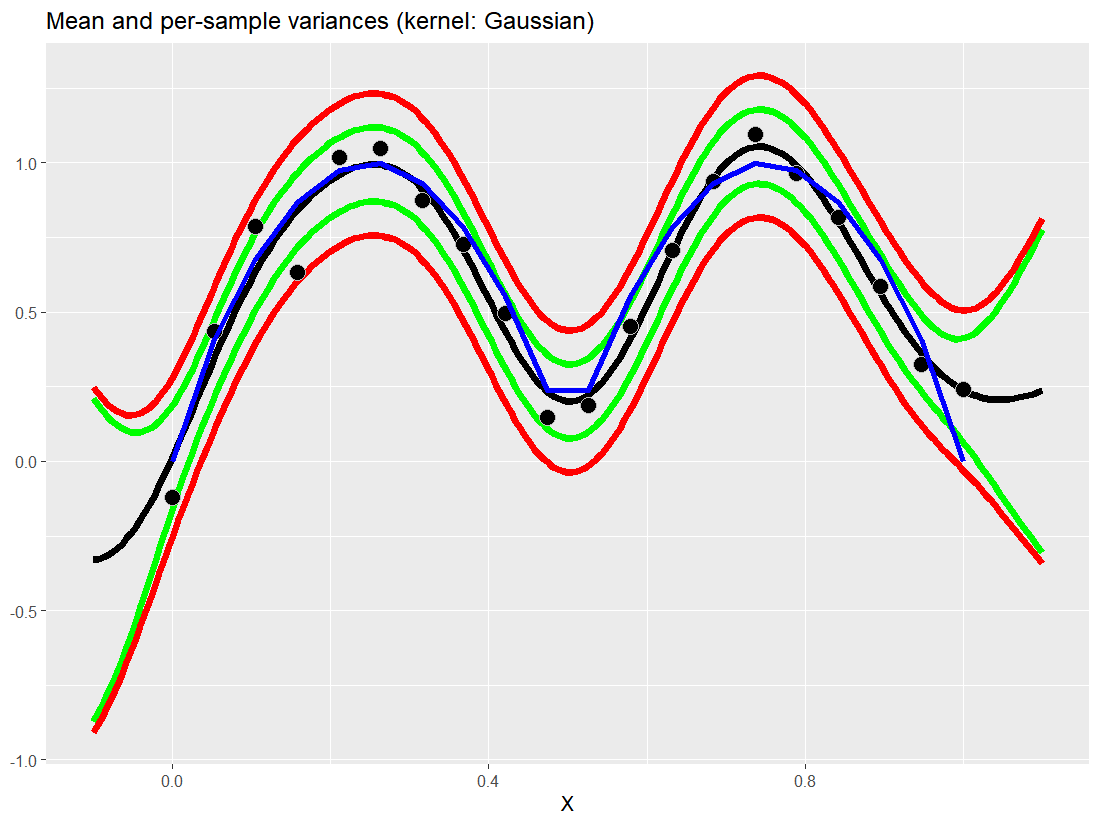
\includegraphics[height=0.5\textwidth]{gaussian_variances.png}
    \caption{
        Plot of a Gaussian process using SE applied to a toy dataset. The toy dataset ($n = 15$) is a data-generating function in blue with some Gaussian noise applied to produce the datapoints in black. The black line represents the expected function from the Gaussian process. The green line represents the 90\% confidence interval around the predictive distribution without the $\sigma^2_n$ term, representing the uncertainty surrounding predictions of the noise-free mean function $f(X)$. The red line represents the 90\% confidence interval with $\sigma^2_n$, representing the uncertainty surrounding predictions of the noisy observations $y$. \\
        TODO explain
    }
\end{figure}

\begin{figure}[H]
    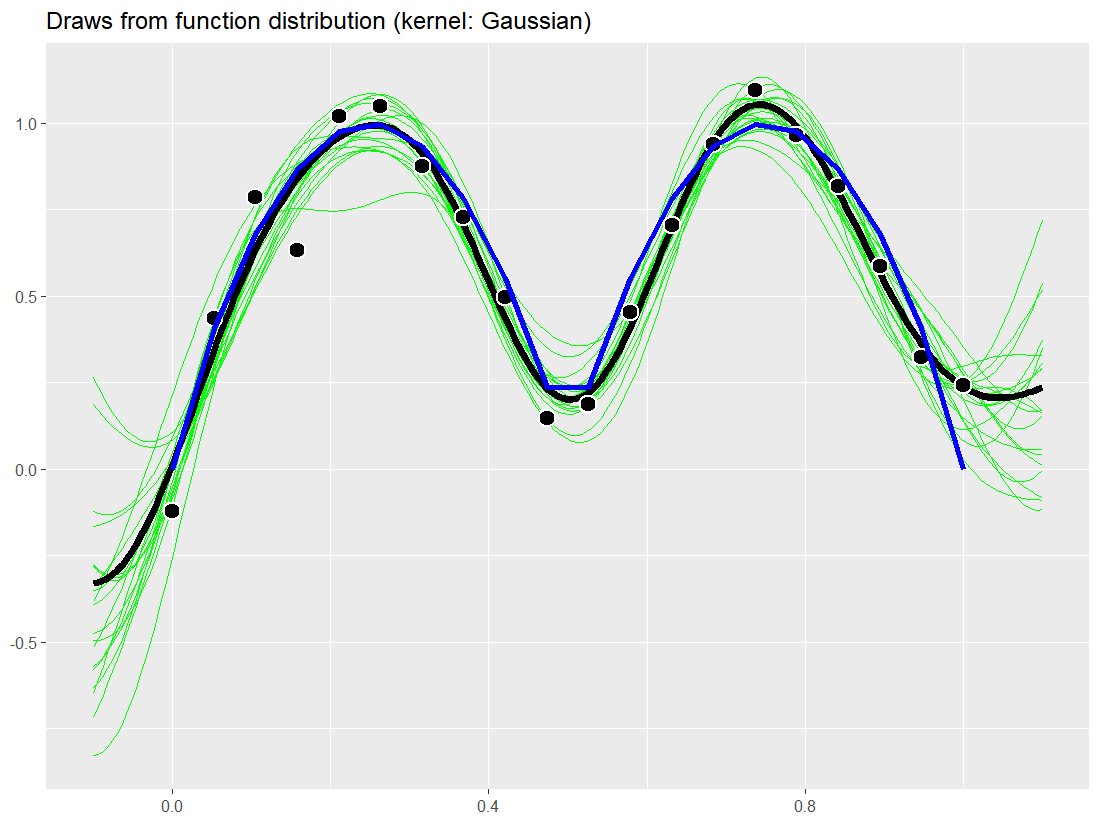
\includegraphics[height=0.5\textwidth]{gaussian_draws.png}
    \caption{
        Plots of functions from a Gaussian process using SE applied to the same toy dataset. The blue line and black datapoints and lines are as before, but the green lines here are a sample of functions drawn from the Gaussian process. \\
        TODO explain
    }
\end{figure}

% Often causes issues since it assumes infinite differentiability. Experts don’t recommend using it. \cite{gaupro}


\subsubsection{Rational quadratic (RQ)}
RQ controls smoothness by using a mixture of different length scales to capture multiple trends in the data with different frequencies. 
\begin{equation*}
    k(X,X') = \left( 1 + \frac{|X - X'|^2}{2\alpha l^2} \right)^{-\alpha}
\end{equation*}
We can derive this form by creating an infinite sum of different instances of SE with a vector of different length-scales $l$ and some weights $w_i$ attached to each instance:
\begin{equation*}
    k(X,X') = \sum_{i=1}^{\infty} w_i \exp \left( -\frac{|X - X'|^2}{2l_i^2} \right)
\end{equation*}
This is a valid covariance function long as the sum remains less than $\infty$ to maintain PSD. We can turn this into a continuous representation if our $l$ is very dense, where $p(l)$ is the PDF for $l$:
\begin{equation*}
    k(X,X') = \int_{0}^{\infty} p(l) \exp \left( -\frac{|X - X'|^2}{2l^2} \right) dl
\end{equation*}
Defining $\tau= l^{-2}$, $l = \tau^{-1/2}$. Putting this into SE:
\begin{equation*}
    k_{SE}(X,X') = \exp(-\frac{|X - X'|^2}{2[\tau^{-1}]}) = \exp(-\frac{1}{2} \tau |X - X'|^2)
\end{equation*}
Before putting this back into the above integral which is in terms of $l$, we need to account for the change of variables from $l$ to $\tau$. The Jacobian factor of this transformation is:
\begin{equation*}
    | \partial_{\tau} l | = \frac{1}{2} \tau^{-3/2} d\tau
\end{equation*}
Defining the transformation $l(x) = \frac{1}{\sqrt{x}}$, putting these into the integral changes the PDF from $p(l)$ to $p(l(\tau)) | \partial_{\tau}l |$:
\begin{equation*}
    k(X,X') = \int_{0}^{\infty} p(l(\tau)) \frac{1}{2} \tau^{-3/2} \exp \left( -\frac{1}{2} \tau |X - X'|^2 \right) d\tau
\end{equation*}
We need an expression for the PDF $p(\tau)$ that integrates to $1$ and is PSD. A common choice is the Gamma distribution with shape $\alpha$ and scale $\beta$ parameters: $\tau \sim \Gamma(\alpha, \frac{\beta}{\alpha})$ 
\begin{equation*}
    p(\tau) \propto \tau ^{\alpha - 1} \exp \left( - \frac{\alpha}{\beta} \tau \right)
\end{equation*}
Putting this into the integral:
\begin{equation*}
    k(X,X') \propto \int_{0}^{\infty}  \left[ \tau^{\alpha - 1} \exp \left(-\frac{\alpha}{\beta} \tau \right) \right] \frac{1}{2}\tau^{-3/2} \exp \left( \tau - \frac{1}{2} \tau |X - X'|^2 \right) d\tau
\end{equation*}
$\frac{1}{2}\tau^{-3/2}$ from $dl$ and the new $\tau^{a-1}$ combine, and the new exponential joins the existing one:
\begin{equation*}
    k(X,X') \propto \int_{0}^{\infty} \frac{1}{2} \tau^{\alpha - \frac{5}{2}} \exp \left[ -\tau \left( -\tau\frac{\alpha}{\beta} + \tau \frac{|X - X'|^2}{2} \right) \right] d\tau
\end{equation*}
We can use the Gamma integral here, but need some rearranging. Absorbing $\frac{1}{2}$ into the proportionality, setting $a = \alpha - \frac{3}{2}$ and factoring $\tau$ out of the exponent for $c = \frac{\alpha}{\beta}\tau + \frac{|X - X'|^2}{2}$:
\begin{equation*}
    k(X,X') \propto \int_{0}^{\infty} \tau^{a - 1} \exp ( -\tau c ) d\tau
\end{equation*}
Applying the Gamma integral and absorbing $\Gamma(a)$ into proportionality:
\begin{equation*}
    k(X,X') \propto c^{-a} \Gamma(a) \propto \left[ \frac{\alpha}{\beta} + \frac{|X - X'|^2}{2} \right]^{-\left( \left[ \alpha - \frac{3}{2} \right] \right)} 
\end{equation*}
Now we need to decide on the parameter values of our Gamma distribution. Since the Gamma distribution strictly takes in one Typically, $\beta = l^-2$ such that $\beta^{-1} = l^2$ and $\frac{\alpha}{\beta} = a \cdot \beta^{-1} = \alpha l^2$. Substituting:
\begin{equation*}
    k(X,X') = \left( al^2 + \frac{|X - X'|^2}{2} \right)^{-\alpha - \frac{3}{2}}
\end{equation*}
Factoring out $al^2$ and absorbing it into the proportionality constant to get our final form:
\begin{equation*}
    k(X,X') = \left( 1 + \frac{|X - X'|^2}{2\alpha l^2} \right)^{-\alpha - \frac{3}{2}}
\end{equation*}
This derivation starts from the discrete length scale $l$ for illustrative purposes, so includes $\frac{3}{2}$ to account for the change from length scale to $\tau$. In practice, derivations start from $\tau$ so never have to change units and never include the $\frac{3}{2}$ term in the exponent.

RQ is infinitely MS differentiable, so produces infinitely smooth functions no matter what the shape parameter of our distribution of length scales $\alpha$ is. As $\alpha \to \infty$, this distribution becomes sharply peaked at the single analytically chosen length scale $l$ and RQ becomes SE. However, as $\alpha \to 1$, we get a wider spread of length scales so our functions capture trends at different frequencies. 

\begin{figure}[H]
    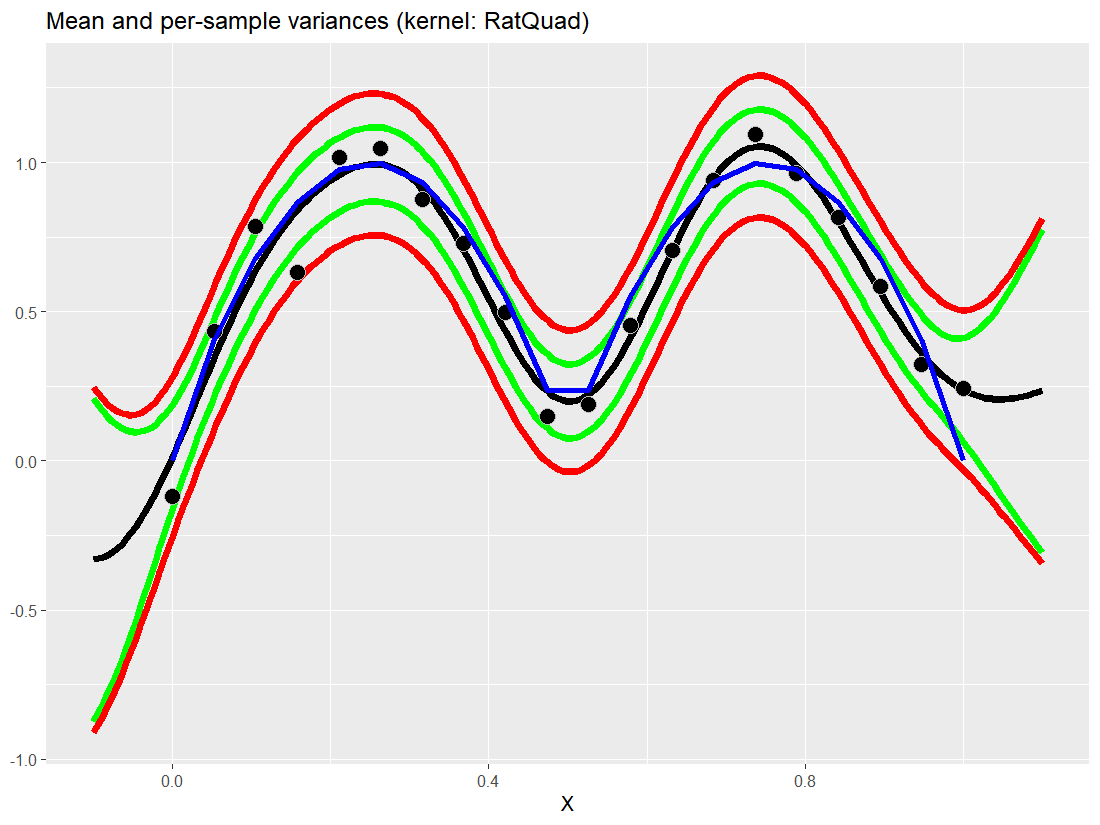
\includegraphics[height=0.5\textwidth]{ratquad_variances.png}
    \caption{
        Plot of a Gaussian process using rational quadratic applied to the toy dataset. For this dataset, the R package GauPro \cite{gaupro} has obtained $\alpha = 100$ via MLE which produces a kernel close to SE, reflecting the lack of trends in this dataset. \\
    }
\end{figure}

\begin{figure}[H]
    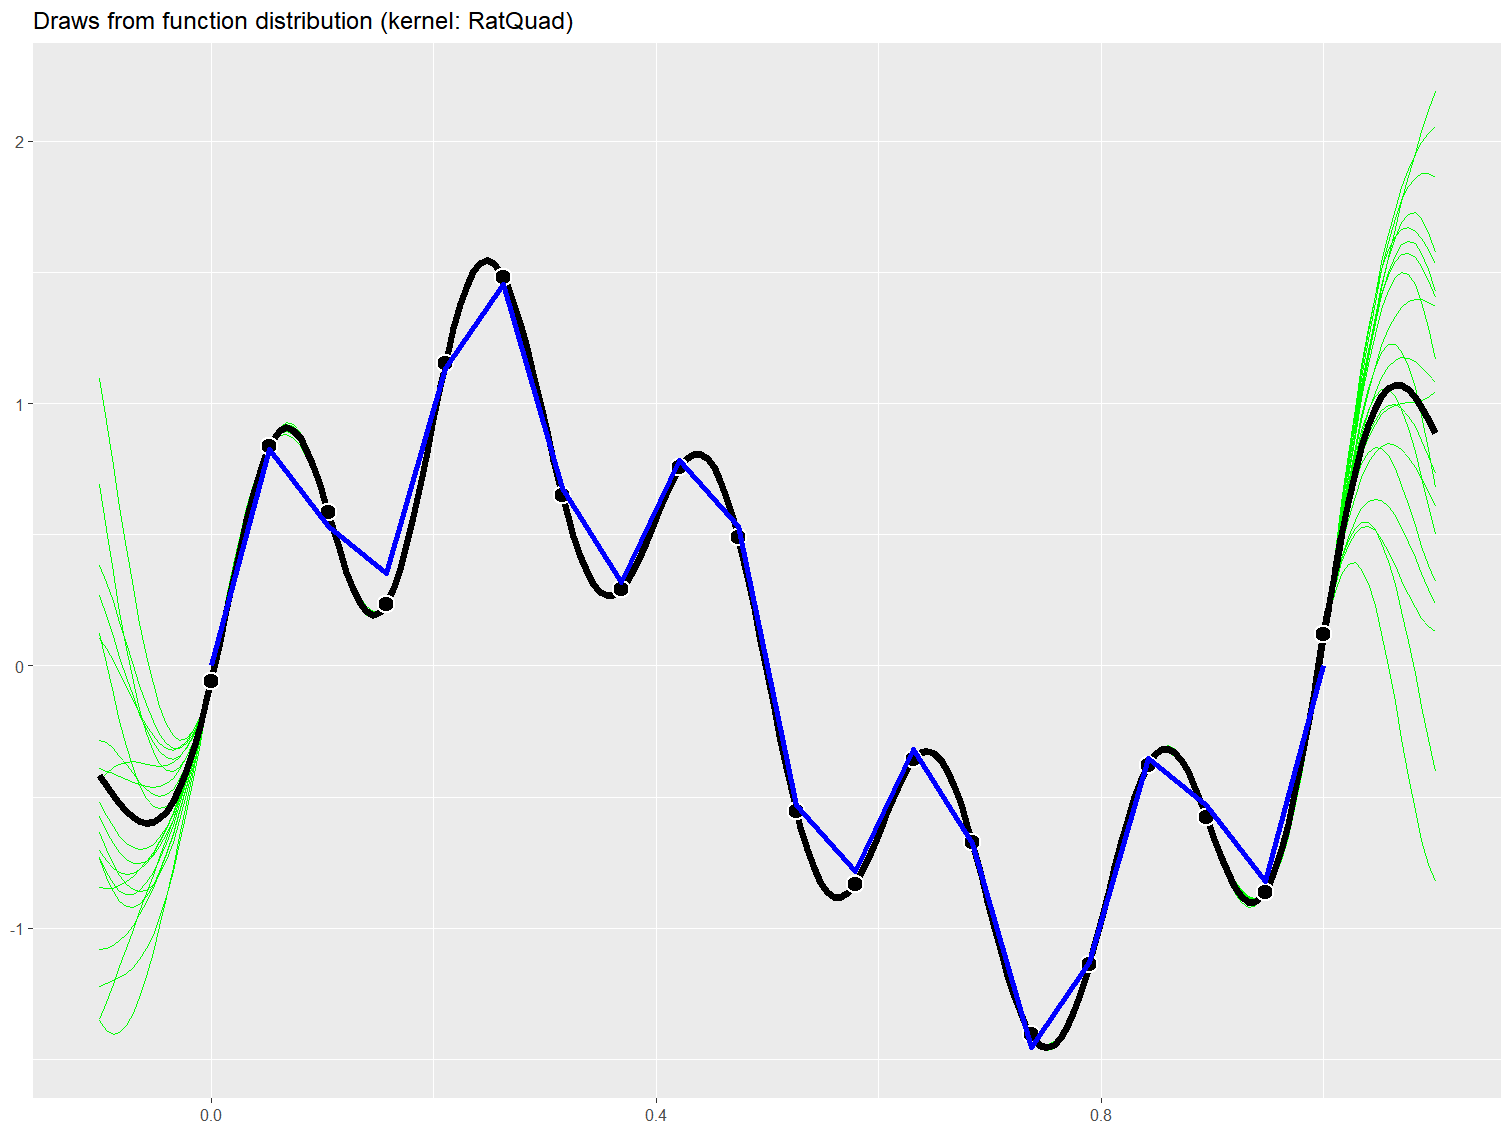
\includegraphics[height=0.5\textwidth]{ratquad_draws.png} \\
    \caption{
        Plots of functions from a Gaussian process using rational quadratic applied to the same toy dataset. \\
    }
\end{figure}

\subsubsection{$\gamma$-exponential and exponential}
SE and RQ have no parameter controlling or reducing its MS differentiability and its smoothness, rendering it a poor approximation of the less smooth functions we often encounter in the real world. We can introduce a differentiability parameter $\gamma$ to control how differentiable the covariance function is:
\begin{equation*}
    k(X,X') = \exp \left(-\frac{|X - X'|^{\gamma}}{l^{\gamma}} \right)
\end{equation*}
where $0 < \gamma \geq 2$ controls the smoothness of the covariance function. 
$\gamma = 2$ produces SE for maximal smoothness. For all other values of $\gamma$ other than $2$, the covariance function is continuous but not differentiable at all at $|x - x'| = 0$, which coincides with the undifferentiable turning point of the modulus function at $x - x' = 0$, and produces the roughest functions of all covariance functions we consider.

\begin{figure}[H]
    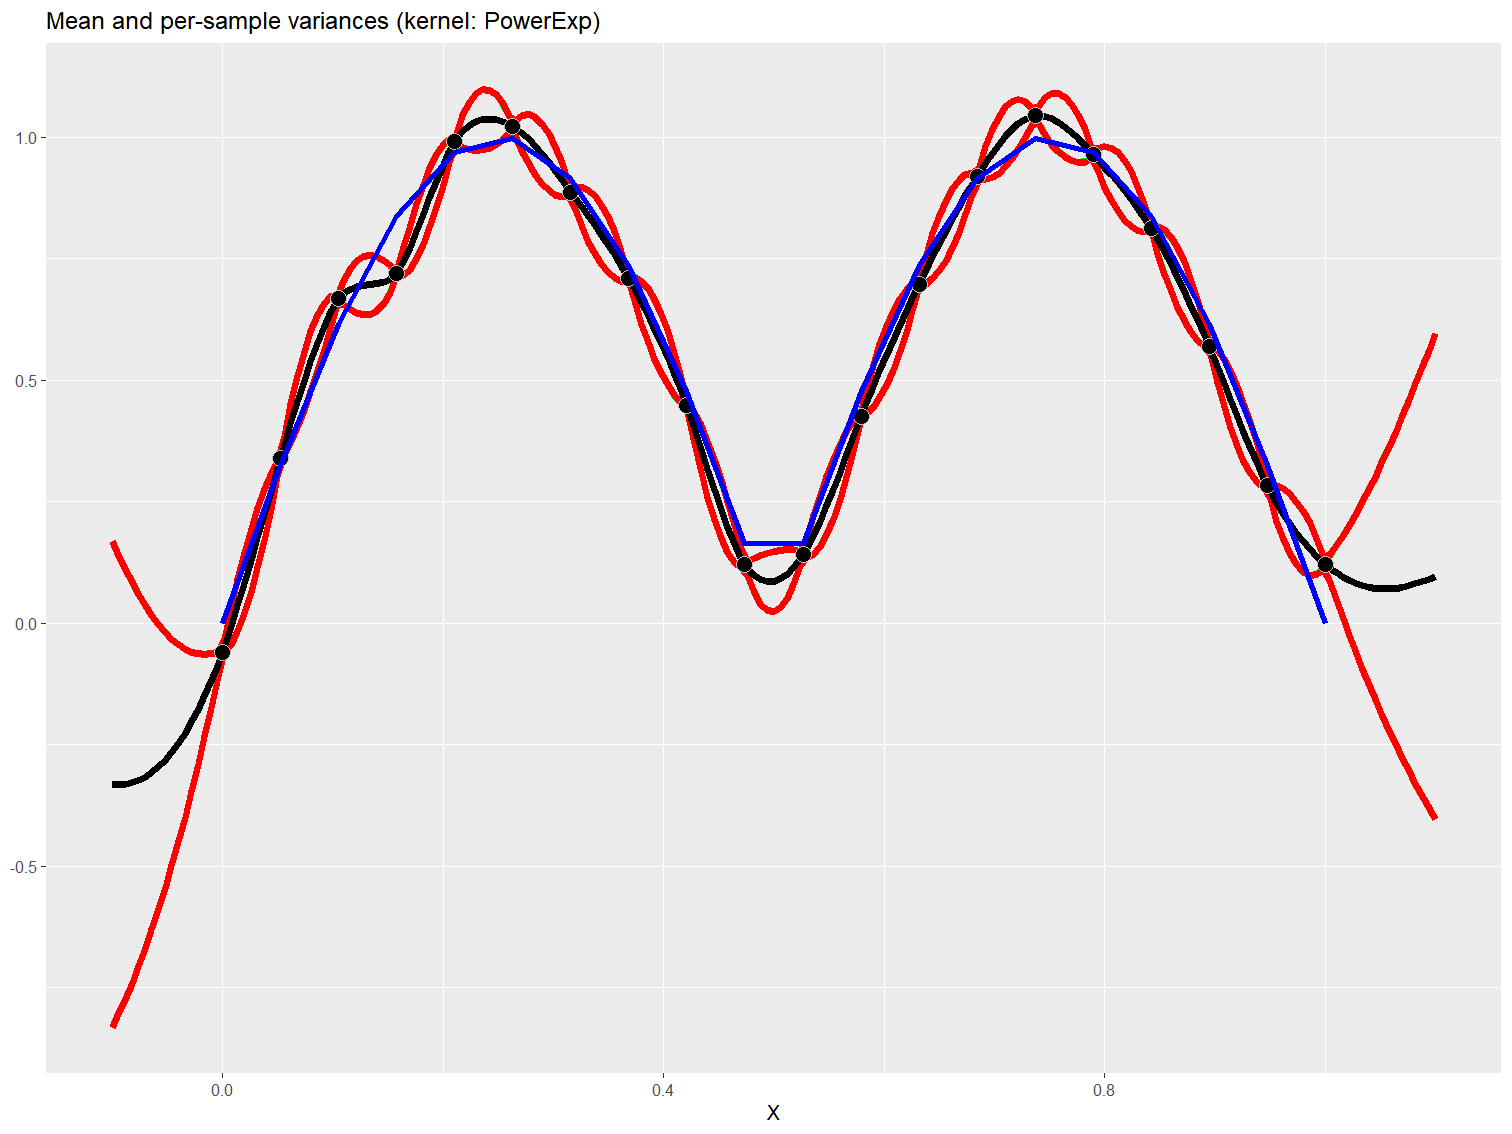
\includegraphics[height=0.5\textwidth]{powerexp_variances.png}
    \caption{
        Plot of a Gaussian process using $\gamma$-exponential applied to the toy dataset. For this dataset, the R package GauPro \cite{gaupro} has used $\gamma = 1.688043$ obtained via MLE. \\
        There are no green lines here because TODO. $\gamma$-exponential produces much rougher functions than SE, so its expected function has a lot more wiggle and conforms to the datapoints much closer than SE. In this case, our data-generating function is smooth so SE is closer to the data-generating function than $\gamma$-exponential, but real world data-generating functions are often much rougher and would benefit from a kernel flexible enough to pass through the datapoints.
    }
\end{figure}

\begin{figure}[H]
    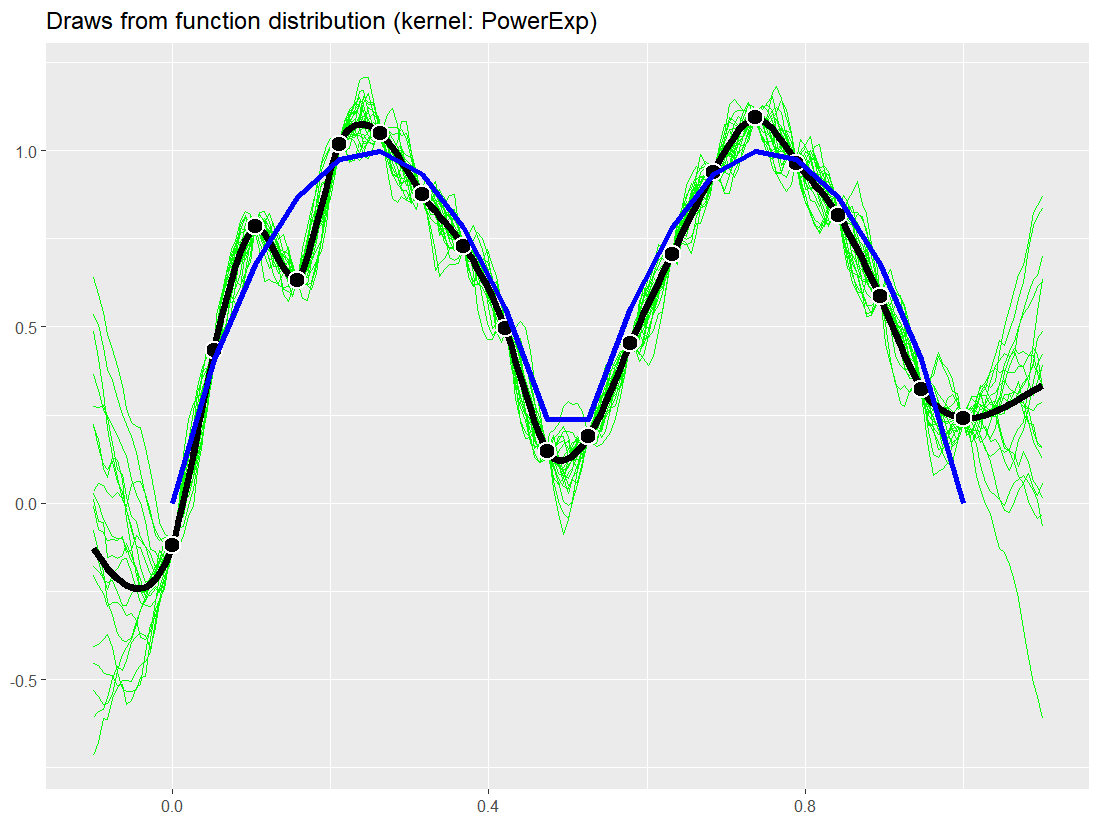
\includegraphics[height=0.5\textwidth]{powerexp_draws.png}
    \caption{
        Plots of functions from a Gaussian process using $\gamma$-exponential applied to the same toy dataset. \\
        These sample function draws are much rougher than SE.
    }
\end{figure}


\paragraph{Exponential covariance function}
$\gamma = 1$ produces the exponential covariance function:
\begin{equation*}
    k(X,X') = \exp \left(-\frac{|X - X'|}{l} \right)
\end{equation*}
Restating:
\begin{equation*}
    k(X, X') = a \exp\left(-c |X - X'|\right)
\end{equation*}
Setting $a = 1$ and $c = \frac{1}{l}$ recovers our familiar exponential kernel \ref{eq:exp_kernel}. Rybicki and Press \cite{fast-exp} showed that any zero-mean GP with this covariance function is the unique stationary solution of the stochastic differential equation (SDE):
\begin{equation*}
    dX_t = -\lambda X_t dt + \sqrt{2\lambda} dW_t
\end{equation*}
TODO explain parts of equation. This corresponds to the form of a strong Markov process:
\begin{equation*}
    dX_t = a(X_t) dt + b(X_t) dW_t
\end{equation*}
TODO explain Markov processes. No other covariance function produces an SDE of order 1.

\begin{figure}[H]
    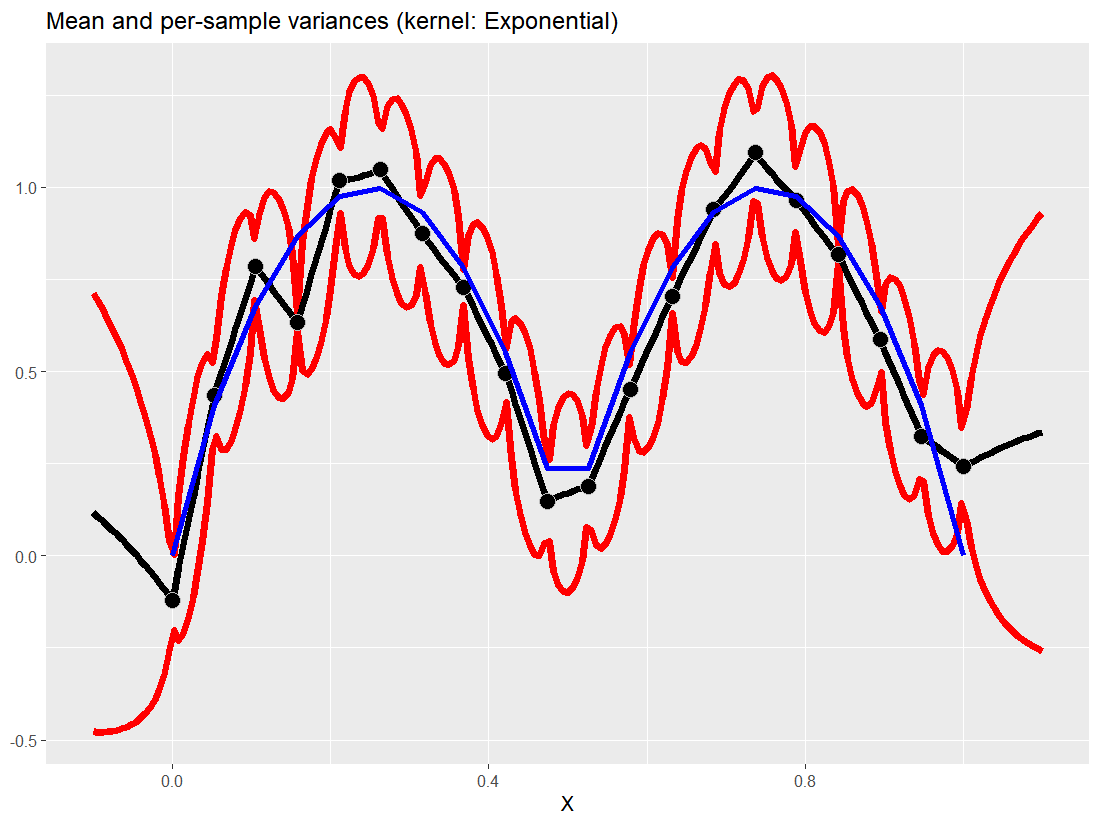
\includegraphics[height=0.5\textwidth]{exp_variances.png}
    \caption{
        Plot of a Gaussian process using exponential applied to the toy dataset. \\
        TODO explain
    }
\end{figure}

\begin{figure}[H]
    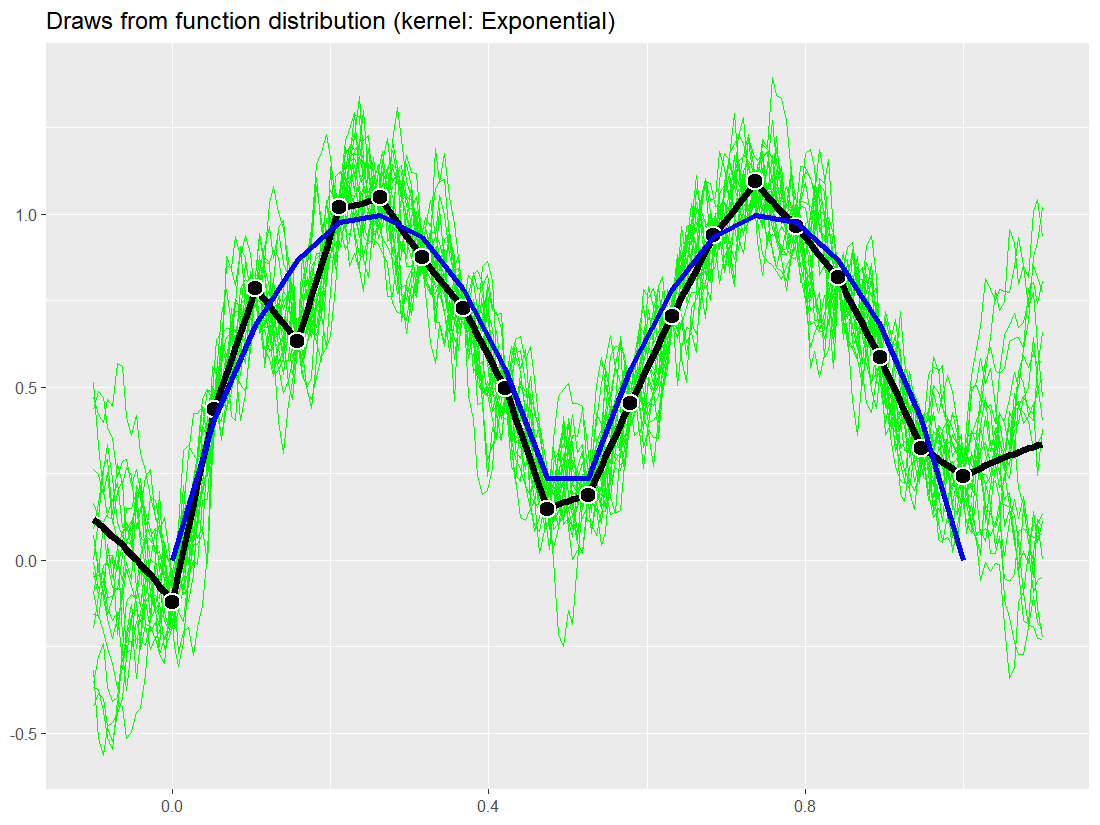
\includegraphics[height=0.5\textwidth]{exp_draws.png}
    \caption{
        Plots of functions from a Gaussian process using exponential applied to the same toy dataset. \\
        These sample function draws are much rougher than SE and $\gamma$-exponential.
    }
\end{figure}


% Exponential: Equivalent to Matern 1/2. Assumes no differentiability. \cite{gaupro}


\subsubsection{Matern-class}
The $\gamma$-exponential generalisation is not useful due to its brittleness - it can only produce two covariance functions representing the extremes of the smoothness-roughness scale. The Matern class of covariance functions addresses this by introducing a parameter $\nu > 0$ that controls the smoothness of the function. The Matern class is defined as:
\begin{equation*}
    k(X,X') = \frac{2^{1 - \nu}}{\Gamma(\nu)}\left(\frac{\sqrt{2\nu}|X - X'|}{l}\right)^{\nu}K_{\nu}\left(\frac{\sqrt{2\nu}|X - X'|}{l}\right)
\end{equation*}

$l$ is our familiar length scale hyperparameter. TODO Bessel function $K_{\nu}$, background needed. Therefore, a Gaussian process using a Matern class kernel is $k$-times MS differentiable if and only if $\nu > k$. 

Using half-integers, i.e. $\nu = p + 1/2$ where $p$ is a non-negative integer, the covariance function becomes a product of a polynomial and an exponential:

\begin{equation*}
    k_{\nu = p + 1/2}(X,X') = \exp \left(- \frac{\sqrt{2\nu}|X - X'|}{l} \right) \frac{\Gamma(p+1)}{\Gamma(2p+1)} \sum_{i=0}^p \frac{(p + i)!}{i!(p-i)!} \left( \frac{\sqrt{8\nu r}}{l} \right)^{p-i}
\end{equation*}

$\nu = 1/2$ is equivelant to the exponential covariance function. As $\nu \to \infty$, the Matern covariance function approaches the SE covariance function. Practically, $\nu \geq 7/2$ produces functions that are as smooth as SE, leaving us with two cases of interest: $\nu = 3/2$ and $\nu = 5/2$.

\paragraph{Matern 3/2}
$\nu = 3/2$ produces the following covariance function:
\begin{equation} \label{eq:matern-32}
    k_{3/2}(X,X') = \left(1 + \frac{\sqrt{3}|X - X'|}{l} \right) \exp \left(-\frac{\sqrt{3}|X - X'|}{l} \right)
\end{equation}
3/2 is one-time MS differentiable, leading to much rougher functions than SE.

\begin{figure}[H]
    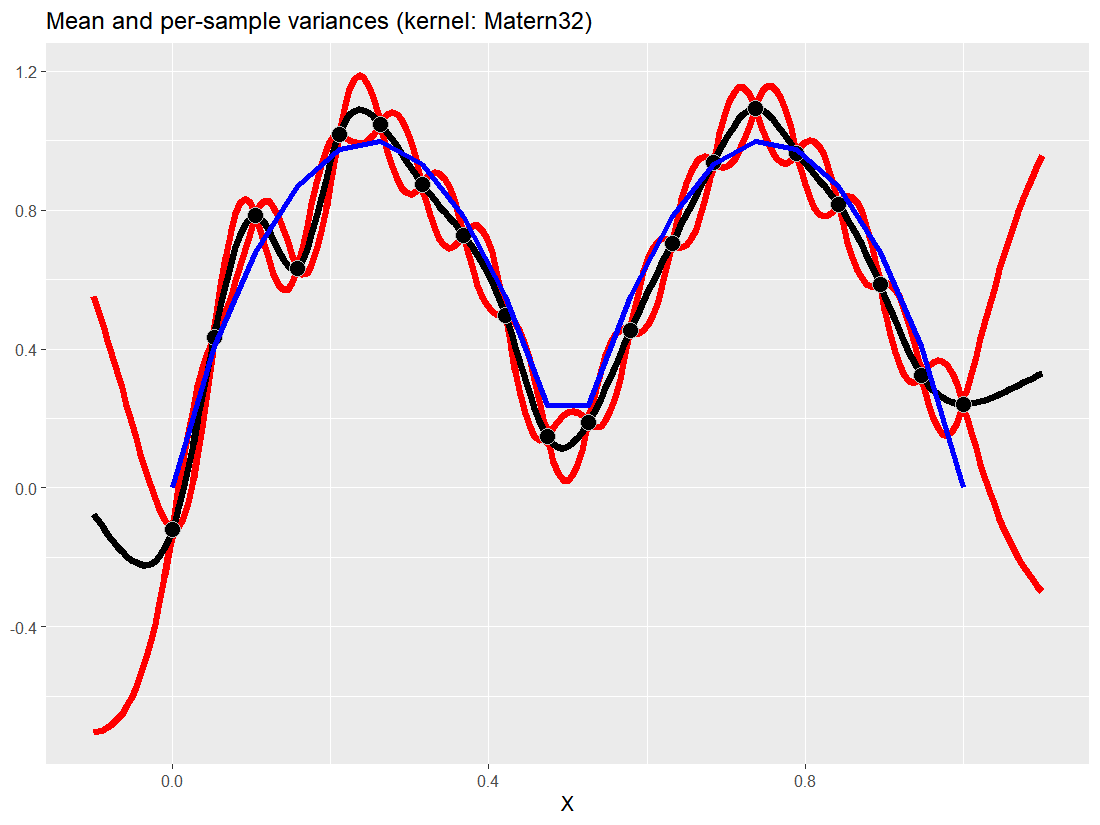
\includegraphics[height=0.5\textwidth]{matern32_variances.png}
    \caption{
        Plot of a Gaussian process using Matern 3/2 applied to the toy dataset. \\
        TODO explain
    }
\end{figure}

\begin{figure}[H]
    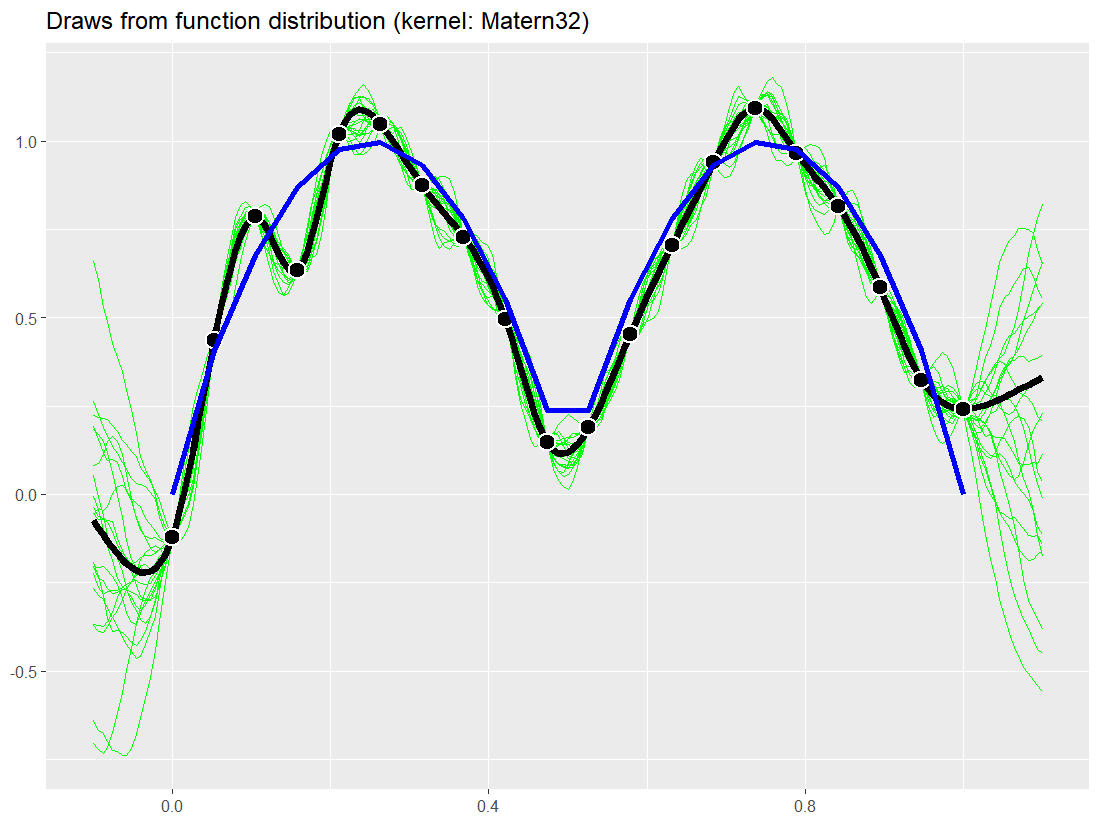
\includegraphics[height=0.5\textwidth]{matern32_draws.png}
    \caption{
        Plots of functions from a Gaussian process using Matern 3/2 applied to the same toy dataset. \\
        TODO explain
    }
\end{figure}

% Matern 3/2: Assumes one time differentiability. This is often too low of an assumption. \cite{gaupro}

\paragraph{Matern 5/2}
$\nu = 5/2$ produces the following covariance function:
\begin{equation*}
    k_{5/2}(X,X') = \left(1 + \frac{\sqrt{5}|X - X'|}{l} + \frac{5|X - X'|^2}{3l^2} \right) \exp \left(-\frac{\sqrt{5}|X - X'|}{l} \right)
\end{equation*}
5/2 is twice MS differentiable, producing functions that are slightly smoother than 3/2.

\begin{figure}[H]
    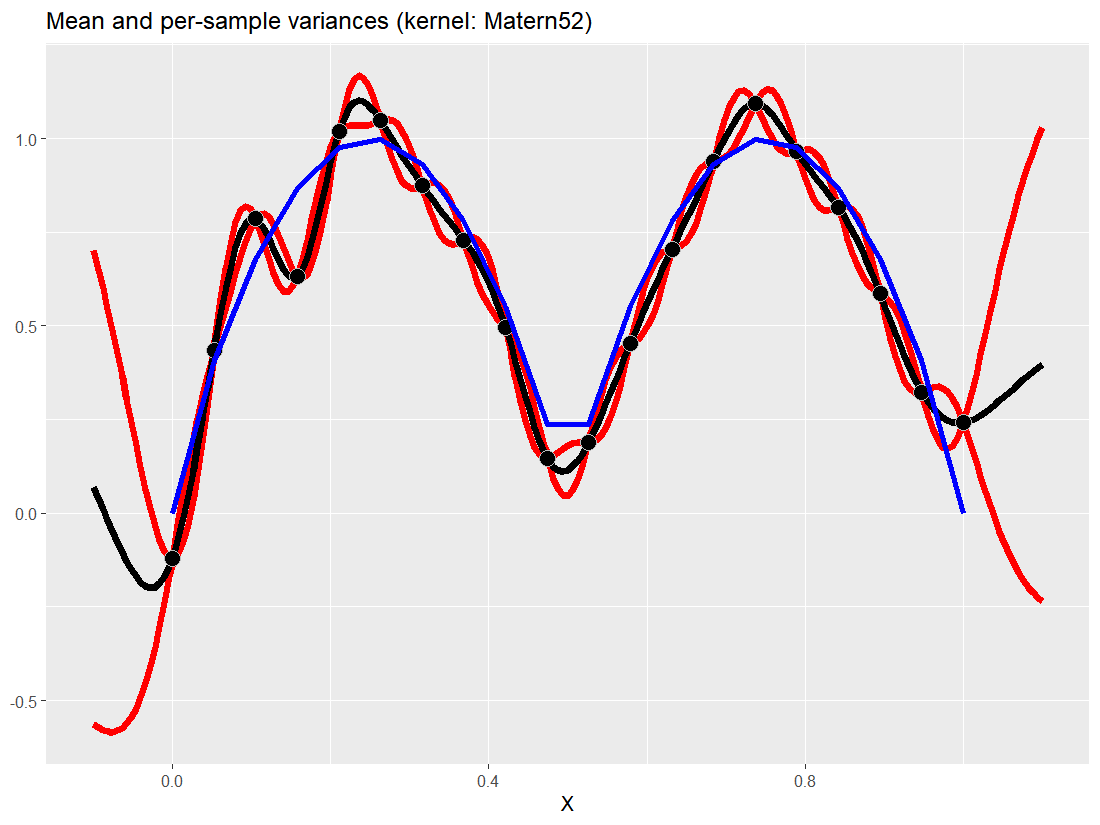
\includegraphics[height=0.5\textwidth]{matern52_variances.png}
    \caption{
        Plot of a Gaussian process using Matern 5/2 applied to the toy dataset. \\
        The expected function deviates very slightly from datapoints compared to 3/2, but the big difference compared to 3/2 is in the variances. 5/2 has narrower variances than 3/2, producing smoother functions and functions that are closer to the expected function. SE is still better in this instance because it is the most smooth and our data-generating function is unusually smooth. However, 5/2 is generally the most popular covariance function because it achieves this parsimonious balance between smoothness, to still reach some reasonable approximation of the data-generating function, and flexibility, to still pass through the datapoints. 
    }
\end{figure}

\begin{figure}[H]
    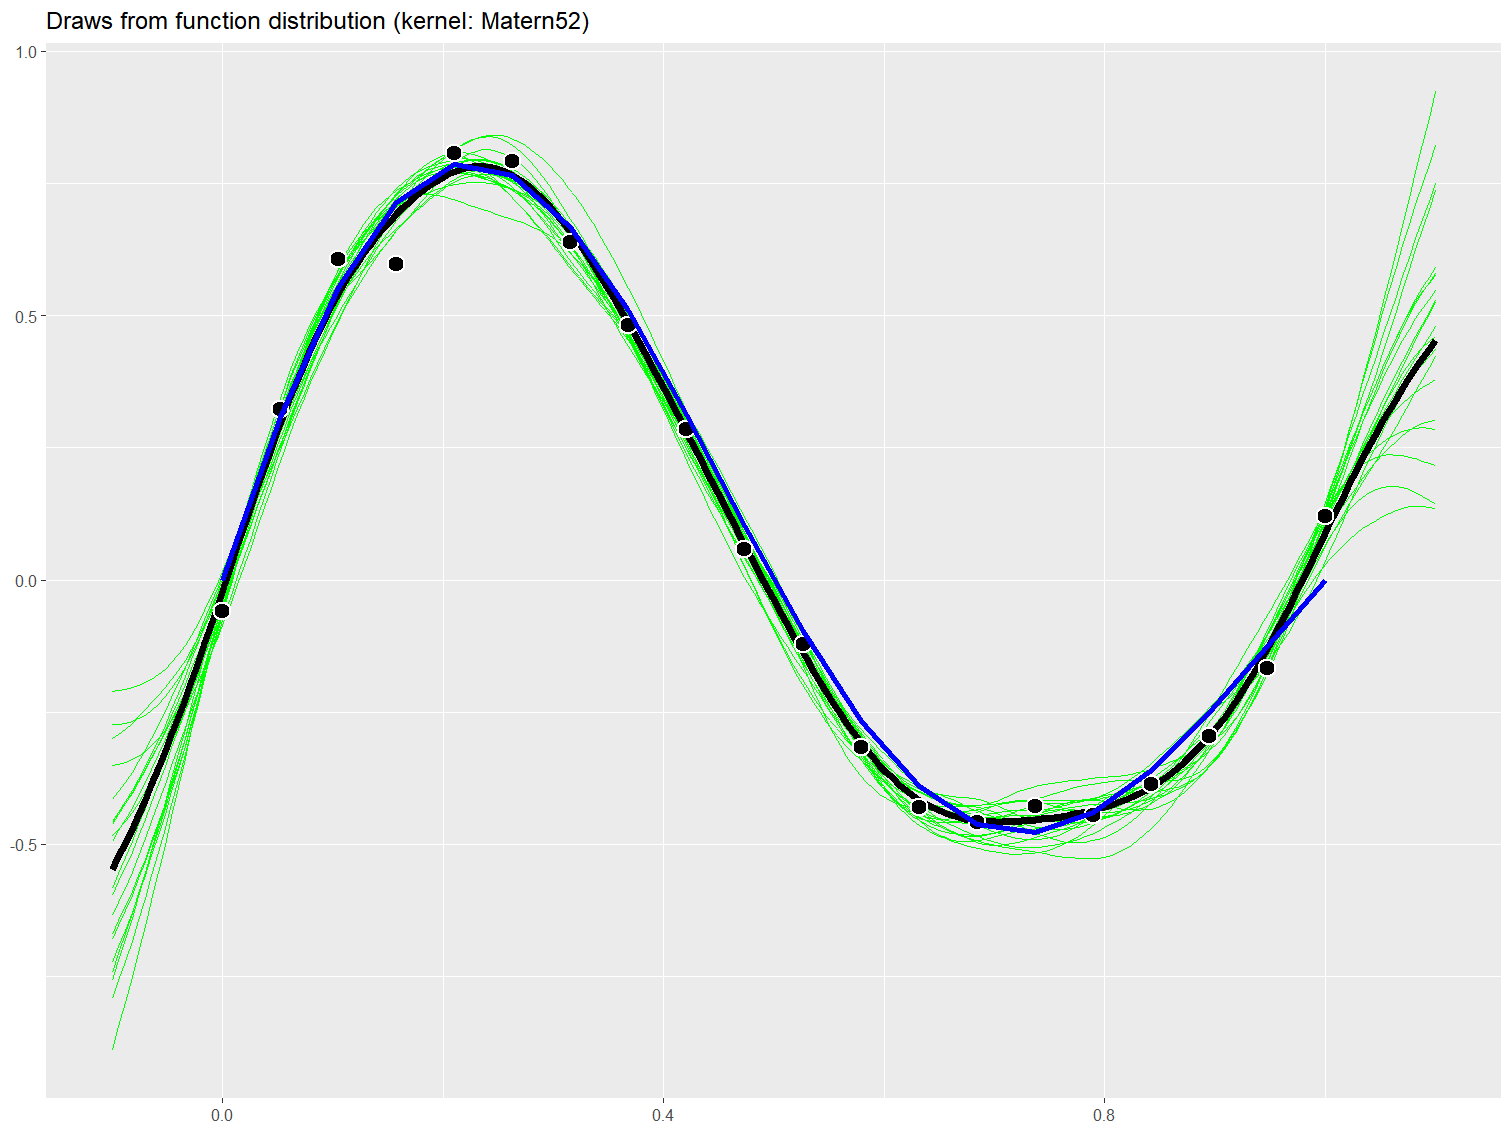
\includegraphics[height=0.5\textwidth]{matern52_draws.png}
    \caption{
        Plots of functions from a Gaussian process using Matern 5/2 applied to the same toy dataset. \\
        These sample function draws conform more to the expected function than 3/2 due to the narrower variances, but are still much rougher than SE and approach the data-points.
    }
\end{figure}

% Matern 5/2: Assumes two time differentiability. Generally the best. \cite{gaupro}




% \subsection{Non-stationary covariance functions \cite{gp-ml}}
% 
% \subsubsection{Sum and product}
% 
% \subsubsection{Neural network}
% 
% \subsubsection{Warping and periodicity}


% \subsection{Language-processing covariance functions \cite{gp-ml}}
% 
% \subsubsection{String}
% 
% \subsubsection{Fisher}
% 
% 
% \subsection{Factor-processing covariance functions \cite{gaupro}}
% 
% \subsubsection{Ordered factor}
% 
% \subsubsection{Factor}
% 
% \subsubsection{Gower factor}
% 
% \subsubsection{Indices-ignoring}


% \subsection{Deriving kernels \cite{deriving-kernels}}
% 
% \subsection{Learning best kernel from data \cite{choosing-kernels}}

% \subsection{Additive covariance kernels for high-dimensional learning \cite{additive-kernels}}
% 
% 
% \subsection{Hierarchical Bayesian covariance function for hierarchical modelling \cite{hierarchical-kernels}}
% 
% 
% \subsection{Free-form covariance matrix for multi-task learning \cite{freeform-kernels}}
% 
% 
% \subsection{Combining different kernels for multi-task learning \cite{multi-kernels}}



% \section{Extensions of the Gaussian Process}
% 
% 
% \subsection{Gaussian process regression networks \cite{gprn}}
% 
% 
% \subsection{Variational Gaussian process \cite{vgp}}
